\documentclass[a4paper]{article}
\usepackage[utf8]{inputenc}
\usepackage{amsmath}
\usepackage{amsfonts}
\usepackage{graphicx}
\usepackage{amssymb}
\usepackage[
	top=3cm,
	bottom=4cm,
	]{geometry}
\setlength{\parindent}{0in}
\usepackage{fancyhdr}

\begin{document}

\pagestyle{fancy}
\rhead{David Nápravník - přezdívka ":)"}

\setcounter{section}{3}
\section{du}
\subsection{chordy}
vyznaceni na grafu $K_6$\\
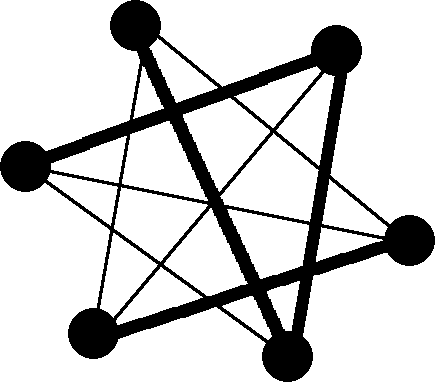
\includegraphics[width=.3\textwidth]{chords.png}\\
pro $n\geq7$ bychom do grafu, kde $n=6$, museli pridat vrchol,
jez by nevytvarel zadnou jednobarevnou kruznici.\\
\textit{Pozorovani:} tento novy vrchol bude stupne 5
a budou existovat pouze dva vrcholy,
se kterymi nebude mit spolecnou hranu.\\
V nasem grafu mame 3 komponenty dle barevnych hran.
A pri pokusu o pridani hran z noveho vrcholu snadno nahledneme,
ze muzeme vynechat pouze dva vrcholi, ale potrebujeme jich tri ... 
pro kazdou komponentu jednu, tudiz at vybereme vrcholi jakkoliv tak
se vzdy jedna z komponent stane cyklem.


\setcounter{subsection}{2}


\subsection{abeceda}
zadane: ~ ~	1123, 2231, 3312, 2311, 3122, 1233\\
dodatecne:~	1132, 2213, 3321, 3211, 1322, 2133, 1111, 2222



\end{document}